\documentclass[letterpaper,11pt]{article}
\usepackage[spanish]{babel}
\usepackage[utf8]{inputenc}
\usepackage{graphicx}
\usepackage{amsfonts,amsmath,amssymb,float, amsthm,mathrsfs}  
\usepackage[right=4.5cm,left=2cm,top=3cm,bottom=3cm,headsep= 0.7cm,footskip=0.5cm]{geometry}
\usepackage{enumerate}
\usepackage{wrapfig} 
\usepackage[rflt]{floatflt} 
\usepackage{framed}
%\usepackage[most]{tcolorbox}
\usepackage[dvipsnames]{xcolor}
\colorlet{shadecolor}{green!20}
\setlength\FrameSep{0.5ex}
\usepackage{thmtools}
\usepackage{esint}
\usepackage{cancel}
\usepackage{listings} 
\usepackage{pstricks, caption}
\usepackage[colorlinks]{hyperref}
\usepackage{csquotes}
\usepackage{fullpage}
\usepackage{enumitem}
\usepackage{etoolbox}
\usepackage{tikz}
\usepackage{tikz-3dplot}
\tdplotsetmaincoords{80}{70}
\usetikzlibrary{decorations.markings}
\usetikzlibrary{arrows,babel}
\usepackage[font=small]{caption}
\usepackage{scalerel} %\scaleto{text}{size}
\usepackage{subfigure}
\usepackage{fancyhdr}
\usepackage{comment}
\usepackage{marginnote}
\usepackage{tensor}
\usepackage{cleveref}
\newcommand{\dbar}{\mathchar'26\mkern-12mu d}
\renewcommand*{\marginnotevadjust}{-0.1cm}
\renewcommand*{\marginfont}{\footnotesize}
\setlength{\headheight}{15pt}
\addtolength{\topmargin}{-14.49998pt}
\setlength{\headsep}{15pt}
\setlength{\footskip}{14.49998pt}
\decimalpoint
\newcommand{\grad}{^\circ}
\newlength{\drop}
\DeclareMathOperator{\sign}{sgn}
\DeclareMathOperator{\Log}{Log}
\providecommand{\norm}[1]{\lVert#1\rVert}

\let\cancelorigcolor\CancelColor% Just for conveniency...

\newcommand{\CancelTo}[3][]{%
  \ifblank{#1}{}{%
    \renewcommand{\CancelColor}{#1}%
  }
  \cancelto{#2}{#3}% 
}


\begin{document}

\pagestyle{plain}

\begin{flushleft}\vspace{-2cm}
Departamento de Física \\
Facultad de Cs. Físicas y Matemáticas\\
Universidad de Concepción
\end{flushleft}

\begin{flushright}\vspace{-1.5cm}
\textbf{Tópicos en Relatividad General} 
\end{flushright}



\rule{\linewidth}{0.1mm}

\begin{center}
\textbf{\LARGE Semana 5}
\end{center}

\begin{flushleft}
\textbf{Nombre:} Alejandro Saavedra San Martín. \\
\textbf{Profesor:} Guillermo Rubilar Alegría.
\end{flushleft}

\section*{Desvío de la luz}

El cálculo es similar al hecho para geodésicas tipo tiempo. Sin embargo, para geodésicas tipo luz no podemos parametrizar la trayectoria con el tiempo propio, sino con un parámetro arbitrario $\lambda$. Así, la ecuación de la geodésica adopta la forma
\begin{equation}
    \frac{d^2 x^{\mu}}{d\tau^2} + \Gamma\indices{^\mu_{\nu \lambda}} \frac{dx^{\nu}}{d\tau} \frac{dx^{\lambda}}{d\tau} = f(\lambda) \frac{dx^{\mu}}{d\lambda}.
\end{equation}

Usando los cálculos hechos en la semana 2, las ecuaciones de las geodésicas adoptan la forma
\colorlet{shadecolor}{green!20}
\begin{shaded}
\begin{align}
\frac{1}{\left(1 - \frac{2m}{r}\right)} \frac{d}{d\lambda}\left[\left( 1 - \frac{2m}{r} \right) \dot{t}\right] &= f \dot{t}, \label{eq:geod-null-1} \\    \Ddot{r} + \frac{mc^2(r-2m)}{r^3} \dot{t}^2 - \frac{m}{r(r-2m)} \dot{r}^2 - (r-2m) \left[\dot{\theta}^2 + \sin^2\theta \dot{\varphi}^2 \right]  &= f \dot{r}, \label{eq:geod-null-2} \\
\Ddot{\theta} + \frac{2}{r} \dot{r} \dot{\theta} - \sin\theta\cos\theta \dot{\varphi}^2 &= f\dot{\theta}, \label{eq:geod-time-3} \\
\frac{1}{r^2\sin^2\theta} \frac{d}{d\lambda} \left[r^2\sin^2\theta \dot{\varphi} \right] &= f \dot{\varphi}, \label{eq:geod-null-4}
\end{align}
\end{shaded}
donde denotamos $\dot{()} := d()/d\lambda$ y se factorizó el lado izquierdo de las ecuaciones \eqref{eq:geod-null-1} y \eqref{eq:geod-null-4} al igual que en la semana 2 pero haciendo el cambio $\tau \to \lambda$. 

El movimiento está confinado a un plano, que podemos elegir como el plano escuatorial, es decir, $\theta(\lambda) = \pi/2$. Claramente esta solución satisface la ecuación \eqref{eq:geod-time-3}. Como nos centraremos en la trayectoria. elegimos como parámetro $\lambda$ el ángulo $\varphi$. Con esto, $\dot{\varphi} = 1$ y podemos determinar $f$ a partir de la ecuación \eqref{eq:geod-null-4}:
\begin{equation}
\frac{1}{r^2\sin^2\left(\frac{\pi}{2}\right)} \frac{d}{d\lambda} \left[r^2\sin^2\left(\frac{\pi}{2}\right) \dot{\varphi} \right] = f \dot{\varphi} \Rightarrow f = \frac{1}{r^2} \frac{d}{d\varphi}[r^2] = \frac{2r}{r^2} \frac{dr}{d\varphi} = \frac{2}{r} \varphi',
\end{equation}
donde hemos denotado $()':=d()/d\varphi$.

Introduciendo esta función $f$ en \eqref{eq:geod-null-1}, obtenemos 
\begin{equation}
\frac{1}{\left(1 - \frac{2m}{r}\right)} \frac{d}{d\varphi}\left[\left( 1 - \frac{2m}{r} \right) t'\right] - \frac{2}{r} t' \varphi' = 0. \label{eq:null-geod-5}
\end{equation}

Luego, si calculamos
\begin{align}
\frac{d}{d\varphi}\ln\left[ \frac{r^2}{\left( 1 - \frac{2m}{r}\right)t'} \right] &= \frac{\left( 1 - \frac{2m}{r}\right)t'}{r^2} \frac{d}{d\varphi}\left[ \frac{r^2}{\left( 1 - \frac{2m}{r}\right)t'} \right] \nonumber\\
&= \frac{\left( 1 - \frac{2m}{r}\right)t'}{r^2} \left( \frac{2r r'}{\left( 1 - \frac{2m}{r}\right)t'} - \frac{r^2}{\left( 1 - \frac{2m}{r}\right)^2 t'\,^2} \frac{d}{d\varphi} \left[\left( 1 - \frac{2m}{r} \right)t' \right] \right) \nonumber\\
&= \frac{2r'}{r} - \frac{1}{\left( 1 - \frac{2m}{r} \right)t'} \frac{d}{d\varphi} \left[\left( 1 - \frac{2m}{r} \right)t' \right]\nonumber \\
&= - \frac{1}{t'} \left( - \frac{2}{r} t' \varphi' +  \frac{1}{\left(1 - \frac{2m}{r}\right)} \frac{d}{d\varphi}\left[\left( 1 - \frac{2m}{r} \right) t'\right]\right).
\end{align}

Usando la ecuación \eqref{eq:null-geod-5}, hemos encontrado que
\begin{equation}
\frac{d}{d\varphi}\ln\left[ \frac{r^2}{\left( 1 - \frac{2m}{r}\right)t'} \right] = 0.
\end{equation}

La ecuación anterior expresa el hecho que existe una cantidad conservada en el movimiento:
\begin{equation} \label{eq:conserved-quantity}
\frac{r^2}{\left( 1 - \frac{2m}{r}\right)t'} =: \frac{c}{\alpha}.
\end{equation}

Por conveniencia posterior, hemos introducido la constante $\alpha$, la cual debe tener dimensiones $[\alpha] = L^{-1}$, para que el lado derecho de la ecuación tenga dimensiones $L^2T^{-1}$ (pues $c$ es la rapidez de la luz).

Por otro lado, la ecuación radial faltante \eqref{eq:geod-null-2} se reduce a 
\begin{align}
r'' + \frac{mc^2(r-2m)}{r^3} t'\,^2 - \frac{m}{r(r-2m)} r'\,^2 - (r-2m) \left[\CancelTo[\color{blue}]{0}{\dot{\theta}^2} + \sin^2\left( \frac{\pi}{2}\right) \cancelto{1}{\dot{\varphi}}^2 \right]  &= \frac{2}{r} r'\,^2 \\
r'' + \frac{mc^2(r-2m)}{r^3} t'\,^2 - \frac{m}{r(r-2m)} r'\,^2 - (r-2m)  &= \frac{2 r'\,^2}{r} . \label{eq:null-geod-radial}
\end{align}

De la condición $g_{\mu\nu}\dot{x}^{\mu} \dot{x}^{\nu} = 0$, tenemos que
\begin{align}
g_{00} c^2 \dot{t}^2 + g_{11} \dot{r}^2 + g_{22} \dot{\theta}^2 + g_{33} \dot{\varphi}^2 &= 0 \\
\left(1 - \frac{2m}{r} \right) c^2 \dot{t}^2 - \frac{1}{\left( 1- \frac{2m}{r} \right)} \dot{r}^2 - r^2 \CancelTo[\color{red}]{0}{\dot{\theta}^2} - r^2\sin^2\left(\frac{\pi}{2}\right) \cancelto{1}{\dot{\varphi}}^2 &= 0 \\
\left(1 - \frac{2m}{r} \right) c^2 \left(\frac{dt}{d\varphi}\right)^2 - \frac{1}{\left( 1- \frac{2m}{r} \right)} \left(\frac{dr}{d\varphi}\right)^2  - r^2  &= 0. \label{eq:null-geod-6}
\end{align}

Si despejamos $t'$ de la ecuación \eqref{eq:conserved-quantity}, 
\begin{equation} \label{eq:null-geod-7}
\frac{dt}{d\varphi} = \frac{r^2\alpha}{c\left(1 - \frac{2m}{r}\right)}.
\end{equation}

Ahora, si reemplazamos \eqref{eq:null-geod-7} en \eqref{eq:null-geod-6}, podremos expresar $dr/d\varphi$ en términos de $r$ y la constante de movimiento $\alpha$:
\begin{align}
\left(1 - \frac{2m}{r} \right) c^2 \left( \frac{r^2\alpha}{c\left(1 - \frac{2m}{r}\right)}\right)^2 - \frac{1}{\left( 1- \frac{2m}{r} \right)} \left(\frac{dr}{d\varphi}\right)^2  - r^2  &= 0 \\
\frac{\alpha^2r^4}{\left( 1 - \frac{2m}{r}\right)} - \frac{1}{\left( 1- \frac{2m}{r} \right)} \left(\frac{dr}{d\varphi}\right)^2  - r^2 &= 0 \\
\alpha^2r^4 - r'\,^2 - r^2 \left( 1- \frac{2m}{r} \right) &= 0.
\end{align}

Reordenando los términos, hemos encontrado una ecuación para la trayectoria $r = r(\varphi)$ de primer orden,
\colorlet{shadecolor}{green!20}
\begin{shaded}
\begin{equation}
r'\,^2 + r^2 - 2mr-\alpha^2 r^4 = 0. \label{eq:null-geod-8}
\end{equation}
\end{shaded}

Si definimos $u := 1/r$, al derivar con respecto a $\varphi$:
\begin{equation}
\frac{du}{d\varphi} = - \frac{1}{r^2} \frac{dr}{d\varphi} \Rightarrow \frac{dr}{d\varphi} = - \frac{1}{u^2} \frac{du}{d\varphi}.
\end{equation}

Así, la ecuación \eqref{eq:null-geod-8} nos queda
\begin{align}
\frac{1}{u^4} u'\,^2 + \frac{1}{u^2} - \frac{2m}{u} - \frac{\alpha^2}{u^4} &= 0 \\
u'\,^2 + u^2 - 2mu^3 - \alpha^2&= 0.
\end{align}

Reordenando los términos, 
\begin{shaded}
\begin{equation}
u'\,^2 + u^2 = \alpha^2 + 2mu^3. \label{eq:null-geod-9}
\end{equation}
\end{shaded}

Derivando esta ecuación, 
\begin{equation}
2u'u'' + 2uu' = 6mu^2 u',
\end{equation}
llegamos a una ecuación de segundo orden en las derivadas de $u$:
\begin{shaded}
\begin{equation}
u'' + u = 3 m u^2. \label{eq:null-geod-9.1}
\end{equation}
\end{shaded}

La ecuación \eqref{eq:null-geod-9.1}, la cual es consecuencia de la ecuación \eqref{eq:null-geod-9} (para $u' \neq 0$) es equivalente a la ecuación para la dinámica radial \eqref{eq:null-geod-radial}. En efecto, como $u = 1/r$, tenemos que
\begin{align}
u' &= - \frac{r'}{r^2}, \\
u'' &= - \frac{r''}{r^2} + \frac{2r'\,^2}{r^3}.
\end{align}

Reemplazando en \eqref{eq:null-geod-9}, 
\begin{align}
- \frac{r''}{r^2} + \frac{2r'\,^2}{r^3} + \frac{1}{r} &= \frac{3m}{r^2} \\
-r'' + \frac{2r'\,^2}{r} + r &= 3m \\
r'' -r + 3m &= \frac{2r'\,^2}{r} \\
r'' + m - (r-2m) &= \frac{2r'\,^2}{r} \\
r'' + m \textcolor{red}{\left(\frac{r^2 - 2m r}{r^2-2m r}\right)} - (r-2m) &= \frac{2r'\,^2}{r} \\
r'' + m \frac{r^2 - 2m r}{r(r-2m)} - (r-2m) &= \frac{2r'\,^2}{r}.\label{eq:null-geod-9.2}
\end{align}

Usando la ecuación \eqref{eq:null-geod-8}:
\begin{equation}
r^2-2mr = \alpha^2r^4 - r'\,^2. \label{eq:null-geod-9.3}
\end{equation}

Reemplazando \eqref{eq:null-geod-9.3} en \eqref{eq:null-geod-9.2}, tenemos que
\begin{align}
r'' + m \frac{(\alpha^2r^4 - r'\,^2 )}{r(r-2m)} - (r-2m) &= \frac{2r'\,^2}{r} \\
r'' + \frac{m r^3}{r-2m}\alpha^2 - \frac{m}{r(r-2m)} r'\,^2 - (r-2m)&= \frac{2r'\,^2}{r}.\label{eq:null-geod-9.4}
\end{align}

Pero, de la ecuación \eqref{eq:null-geod-7}:
\begin{equation}
\alpha = \frac{c(r-2m)t'}{r^3}. \label{eq:null-geod-9.5}
\end{equation}

Reemplazando \eqref{eq:null-geod-9.5} en \eqref{eq:null-geod-9.4}:
\begin{align}
r'' + \frac{m r^3}{r-2m} \left(\frac{c(r-2m)t'}{r^3} \right)^2 - \frac{m}{r(r-2m)} r'\,^2 - (r-2m)&= \frac{2r'\,^2}{r} \\
r'' + \frac{mc^2(r-2m)}{r^3} t'\,^2 - \frac{m}{r(r-2m)} r'\,^2 - (r-2m) &= \frac{2r'\,^2}{r} 
\end{align}

Probando así la equivalencia entre la ecuación \eqref{eq:null-geod-radial} y \eqref{eq:null-geod-9.1}. Además, al ser \eqref{eq:null-geod-9.1} consecuencia de \eqref{eq:null-geod-9} y \eqref{eq:null-geod-9} de \eqref{eq:null-geod-8}. Hemos probado que la ecuación \eqref{eq:null-geod-8} implica la condición \eqref{eq:null-geod-radial}. 


El término introducido por la teoría de Relatividad General es $3mu^2$. Si tomamos el límite $m\to 0$, obtenemos la ecuación para el caso newtoniano:
\begin{equation} \label{eq:null-geod-10}
u'' + u = 0,
\end{equation}
cuyas soluciones son líneas rectas. En efecto, la solución general de \eqref{eq:null-geod-10} es la de un oscilador armónico libre de frecuencia $\omega_0 = 1$:
\begin{equation}
u_0(\varphi) = \frac{1}{D}\sin(\varphi - \varphi_0),
\end{equation} 
donde $D$ es una constante de integración con dimensiones de longitud y $\varphi_0$ otra constante pero angular. Entonces, la trayectoria en coordenadas cartesianas viene dada por
\begin{align}
x &= r\cos\varphi = D \frac{\cos(\varphi)}{\sin(\varphi-\varphi_0)}, \label{eq:null-geod-x}\\
y &= r\sin\varphi = D \frac{\sin(\varphi)}{\sin(\varphi-\varphi_0)}. \label{eq:null-geod-y}
\end{align}

Encontremos la ecuación de la curva en coordenadas cartesianas, es decir, relacionemos $x$ e $y$ por medio de una ecuación. Primero, desarrollemos
\begin{equation}
\frac{D}{\cos(\varphi_0)} + (\tan(\varphi_0)) x. \label{eq:null-geod-11}
\end{equation}

Reemplazando \eqref{eq:null-geod-x} en \eqref{eq:null-geod-11}:
\begin{align}
\frac{D}{\cos(\varphi_0)} + \tan(\varphi_0) x &= \frac{D}{\cos(\varphi_0)} + \tan(\varphi_0) \frac{D\cos(\varphi)}{\sin(\varphi-\varphi_0)} \nonumber\\
&= D\left[ \frac{1}{\cos(\varphi_0)} + \frac{\sin(\varphi_0)\cos(\varphi)}{\cos(\varphi_0)(\sin(\varphi)\cos(\varphi_0) - \cos(\varphi)\sin(\varphi_0))} \right] \nonumber\\
&= D \frac{\sin(\varphi)\cos(\varphi_0) - \cos(\varphi)\sin(\varphi_0) + \sin(\varphi_0)\cos(\varphi)}{\cos(\varphi_0)(\sin(\varphi)\cos(\varphi_0) - \cos(\varphi)\sin(\varphi_0))}\nonumber \\
&= D \frac{\sin(\varphi)}{\sin(\varphi)\cos(\varphi_0) - \cos(\varphi)\sin(\varphi_0)} \nonumber\\
&= D  \frac{\sin(\varphi)}{\sin(\varphi-\varphi_0)}.
\end{align}

Comparando con \eqref{eq:null-geod-y}, hemos encontrado que las soluciones de \eqref{eq:null-geod-10} son líneas rectas dadas por 
\begin{equation} \label{eq:null-geod-12}
y = \frac{D}{\cos(\varphi_0)} + \tan(\varphi_0) x.
\end{equation}

En particular, la solución \eqref{eq:null-geod-12} es una línea recta en el plano $xy$ de pendiente $\tan(\varphi_0)$ y coeficiente de posición $D/\cos(\varphi_0)$, es decir, la recta intersecta el eje $y$ en el punto $(0,D/\cos(\varphi_0))$. Es fácil de ver de la figura \ref{fig:rayo-luz-newton} que la constante $D$ es la distancia mínima de la recta al origen y $\varphi_0$ el ángulo que forma la recta y el eje $x$.

\begin{figure}
\centering
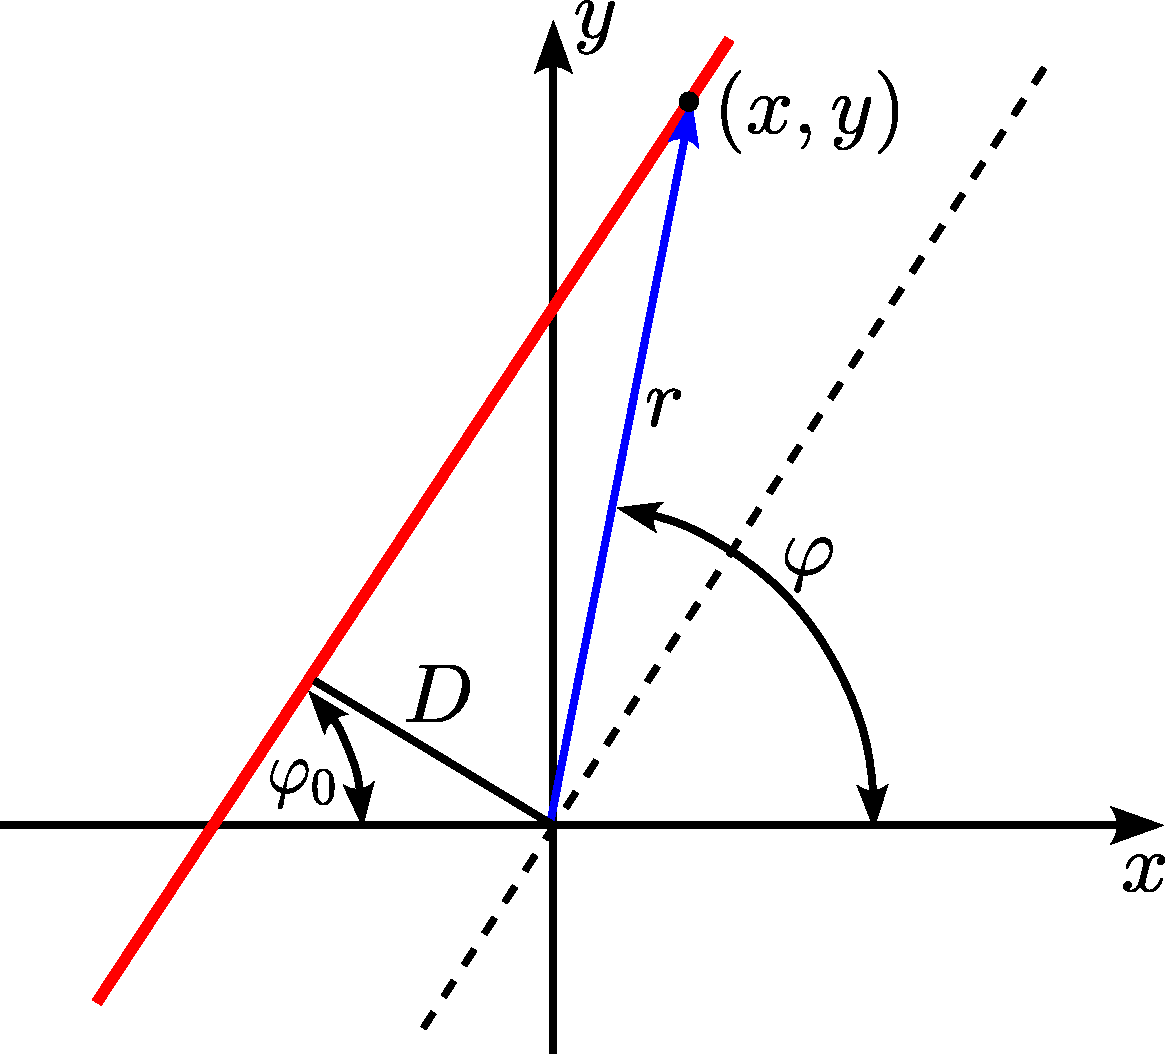
\includegraphics[scale=0.35]{fig-recta}
\caption{Solución newtoniana para el movimiento del rayo de luz. Recuperado del apunte del profesor \href{https://github.com/gfrubi/RG}{Guillermo Rubilar}.}
\label{fig:rayo-luz-newton}
\end{figure}

Similarmente para el caso de geodésicas tipo tiempo, determinemos una solución perturbativa de \eqref{eq:null-geod-9}. Para ello, definamos la variable adimensional $w(\varphi) := D u(\varphi)$, luego reemplacemos en \eqref{eq:null-geod-9}:
\begin{align}
u'' + u &= 3mu^2 \\
\frac{1}{D}w'' + \frac{1}{D} w &= \frac{3m}{D^2} w^2 \\
w'' + w &= \frac{3m}{D} w^2. \label{eq:null-geod-13}
\end{align}

Si definimos la constante
\begin{equation}
\epsilon := \frac{3m}{D},
\end{equation}
la ecuación \eqref{eq:null-geod-13} nos queda
\begin{shaded}
\begin{equation}\label{eq:null-geod-14}
w'' + w = \epsilon w^2.
\end{equation}
\end{shaded}

El parámetro $\epsilon$ es pequeño (mucho menor que 1), ya que suponemos que el rayo de luz pasa suficientemente lejos del centro de fuerzas  de modo que $D \gg m$. Por lo tanto, ocuparemos $\epsilon$ como parámetro perturbativo. 

Usando el método perturbativo, postulamos la siguiente expansión para la solución de \eqref{eq:null-geod-14}:
\begin{equation}
w = w_0(\varphi) + \epsilon w_1(\varphi) + \epsilon^2 w_2(\varphi) + \mathcal{O}(\epsilon^3),
\end{equation}
donde $w_0$ es la solución no perturbada de
\begin{equation}
w_0'' + w_0 = 0,
\end{equation}
la cual corresponde a la ecuación diferencial ordinaria (EDO) de un oscilador armónico libre con solución
\begin{equation}
w_0(\varphi) = \sin(\varphi - \varphi_0).
\end{equation}

Reemplazando la solución perturbada en \eqref{eq:null-geod-14}, obtenemos 
\begin{align}
w'' + w &= \epsilon w^2 \\
w_0'' + \epsilon w_1'' + w_0 + \epsilon w_1 + \mathcal{O}(\epsilon^2) &= \epsilon \left( w_0 + \epsilon w_1 + \mathcal{O}(\epsilon^2)\right)^2 \\
(w_0'' + w_0) + \epsilon (w_1'' + w_1)+ \mathcal{O}(\epsilon^2) &= \epsilon w_0^2 + \mathcal{O}(\epsilon^2) \\
0 + \epsilon(w_1'' + w_1)+ \mathcal{O}(\epsilon^2) &= \epsilon w_0^2 + \mathcal{O}(\epsilon^2).
\end{align}

Igualando los términos de primer orden en $\epsilon$, $w_1$ es solución de la EDO
\begin{align}
w_1'' + w_1 &= w_0^2 \nonumber \\
&= \sin^2(\varphi - \varphi_0)  \nonumber\\
&= \frac{1}{2} - \frac{1}{2}\cos[2(\varphi - \varphi_0)] \label{eq:EDO-w1}
\end{align}
donde se usó la identidad $\sin^2\varphi \equiv (1 - \cos(2\varphi))/2$.

La solución general de esta ecuación es de la forma \footnote{La solución está sobredeterminada, pues al ser la EDO de un oscilador armónico con término forzante constante y otro periódico no resonante, la solución es $w_1(\varphi) = A + B \cos[2(\varphi - \varphi_0)]$.}
\begin{equation}\label{eq:null-geod-sol-pert}
w_1(\varphi) = A + B \cos(\varphi - \varphi_0 + \beta) + C\cos^2(\varphi - \varphi_0).
\end{equation}

Reemplazando en la ecuación \eqref{eq:EDO-w1}:
\begin{align}
w_1'' + w_1 &=  \frac{1}{2} - \frac{1}{2}\cos[2(\varphi - \varphi_0)] \\
\frac{d}{d\varphi} \left[A + B \cos(\varphi - \varphi_0 + \beta) + C \left( \frac{1}{2} + \frac{1}{2} \cos[2(\varphi - \varphi_0)] \right)\right] + w_1 &=  \frac{1}{2} - \frac{1}{2}\cos[2(\varphi - \varphi_0)] \\
- B\cos(\varphi - \varphi_0 +\beta) - 2C \cos[2(\varphi - \varphi_0)] + w_1 &= \frac{1}{2} - \frac{1}{2}\cos[2(\varphi - \varphi_0)] \\
- 2C \cos[2(\varphi - \varphi_0)] + A + \frac{C}{2} + \frac{C}{2} \cos[2(\varphi - \varphi_0)] &= \frac{1}{2} - \frac{1}{2}\cos[2(\varphi - \varphi_0)]  \\
\left(A + \frac{C}{2}\right) -  \frac{3}{2}C \cos[2(\varphi - \varphi_0)] &= \frac{1}{2} - \frac{1}{2}\cos[2(\varphi - \varphi_0)].
\end{align}

Como las funciones $\cos[n(\varphi - \varphi_0)]$, $n = 0,1,2,\dots$ son linealmente independientes, 
\begin{equation}
 A + \frac{C}{2} = \frac{1}{2}, \quad -  \frac{3}{2}C = - \frac{1}{2}.
\end{equation}

Así, hemos encontrado que $A = C = 1/3$, mientras que las constante $B$ y $\beta$ pueden adoptar valores arbitrarios. Eligimos $B = \beta = 0$. Entonces,
\begin{equation}
w(\varphi) = \sin(\varphi - \varphi_0) + \epsilon \left[ \frac{1}{3} + \frac{1}{3}\cos^2(\varphi - \varphi_0)\right] + \mathcal{O}(\epsilon^2).
\end{equation}

Pero, $w(\varphi) = D u(\varphi)$ y $\epsilon = 3m/D$. Por lo tanto, nuestra solución a primer orden adopta la forma:
\begin{shaded}
\begin{equation}\label{eq:null-geod-15}
u(\varphi) = \frac{1}{D} \left[ \sin(\varphi - \varphi_0) + \frac{m}{D} \left[ 1 + \cos^2(\varphi-\varphi_0)\right] \right] + \mathcal{O}(\epsilon^2).
\end{equation}
\end{shaded}

En el siguiente \href{https://github.com/AleSaa66/Topicos-RG/blob/main/Semana%204/Semana-5.ipynb}{notebook} se encuentra un gráfico de la solución \eqref{eq:null-geod-15} para diferentes valores de $\epsilon$ considerando el campo gravitacional producto del Sol.

Para calcular el ángulo de desvío de la luz $\delta$, necesitamos los ángulos $\delta_1$ y $\delta_2$ en que la trayectoria se desvía de la recta no perturbada, para $t \to - \infty$ y $t \to +\infty$, respectivamente, ver figura \ref{fig:rayo-luz-GR}. Estos ángulos corresponden a un ángulo inicial $\varphi_{\text{i}} = \varphi_0 + \pi + \delta_1$ y final $\varphi_{\text{f}} = \varphi_0 - \delta_2$, y pueden ser determinados por la condición que en cada caso $r \to \infty$ o, equivalentemente $u = 0$.
\begin{figure}
\centering
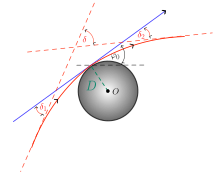
\includegraphics[scale=0.5]{Desvio-Luz}
\caption{Desvío de un haz de luz (curva sólida en rojo) y el haz de luz no perturbado (curva sólida en azul) debido a la curvatura del espacio-tiempo ocasionada por un cuerpo esférico. }
\label{fig:rayo-luz-GR}
\end{figure}

Reemplazando $\varphi = \varphi_{\text{i}}$ en la condición $u(\varphi_{\text{i}}) = 0$, a primer orden en $\delta_1$:\footnote{El ángulo $\delta_1$ está relacionado al parámetro $\epsilon$, pues si varía $\epsilon = 3m/D$, el cual depende de la distancia mínima del rayo de luz al cuerpo esférico de masa $M$, el rayo de luz puede desviarse en mayor o menor medida.}
\begin{align}
0 &= u(\varphi_{\text{i}}) \nonumber \\
&= \frac{1}{D} \left[ \sin(\varphi_0 + \pi + \delta_1 - \varphi_0) + \frac{m}{D} \left[ 1 + \cos^2(\varphi_0 + \pi + \delta_1-\varphi_0)\right] \right] \nonumber \\
&= \frac{1}{D} \left[ \sin(\pi + \delta_1) + \frac{m}{D} \left[ 1 + \cos^2(\pi + \delta_1)\right] \right] \nonumber\\
&= \frac{1}{D} \left[ - \sin(\delta_1) + \frac{m}{D} \left[ 1 + (-\cos(\delta_1))^2\right] \right] \nonumber\\
&= \frac{1}{D} \left[ - \delta_1 + \mathcal{O}(\delta_1^2) + \frac{m}{D} \left[ 1 + (1 + \mathcal{O}(\delta_1^2))^2 \right] \right]\nonumber \\
&= \frac{1}{D} \left[ - \delta_1  + \frac{2m}{D} + \mathcal{O}(\delta_1^2) \right],
\end{align}
donde en la penúltima línea se usó las expansiones en serie de Taylor para el coseno y seno:
\begin{align}
\cos(x) &= 1 - \frac{x^2}{2!} + \frac{x^4}{4!} - \cdots, \\
\sin(x) &= x - \frac{x^3}{3!} + \frac{x^5}{5!} - \cdots . 
\end{align}

Por lo tanto, obtenemos que
\begin{equation}
\delta_1 = \frac{2m}{D}.
\end{equation}

Similarmente, para $\varphi_{\text{f}} = \varphi_0 - \delta_2$, tenemos que
\begin{align}
0 &= u(\varphi_{\text{f}}) \nonumber \\
&= \frac{1}{D} \left[ \sin(\varphi_0 - \delta_2 - \varphi_0) + \frac{m}{D} \left[ 1 + \cos^2(\varphi_0 - \delta_2-\varphi_0)\right] \right] \nonumber \\
&= \frac{1}{D} \left[ \sin( - \delta_2) + \frac{m}{D} \left[ 1 + \cos^2( - \delta_2)\right] \right] \nonumber\\
&= \frac{1}{D} \left[ - \sin(\delta_2) + \frac{m}{D} \left[ 1 + \cos^2(\delta_2)\right] \right] \nonumber\\
&= \frac{1}{D} \left[ - \delta_2 + \mathcal{O}(\delta_2^2) + \frac{m}{D} \left[ 1 + (1 + \mathcal{O}(\delta_2^2))^2 \right] \right]\nonumber \\
&= \frac{1}{D} \left[ - \delta_2  + \frac{2m}{D} + \mathcal{O}(\delta_2^2) \right],
\end{align}

Por lo tanto, obtenemos que
\begin{equation}
\delta_2 = \frac{2m}{D}.
\end{equation}

De la figura \ref{fig:rayo-luz-GR} se observa que $\delta = \delta_1 + \delta_2$. Así, el ángulo de desvío está dado por
\begin{equation}
\delta \approx \frac{4m}{D},
\end{equation}
o, en términos de la masa central $M$,
\begin{shaded}
\begin{equation}\label{eq:desbio-luz}
\delta \approx \frac{4GM}{c^2D}.
\end{equation}
\end{shaded}

En el caso de rayos de luz pasando muy cerca de la superficie del Sol, $D \approx R_{\odot}$, 
\begin{equation}
\delta_{\odot} \approx \frac{4GM_{\odot}}{c^2R_{\odot}}.
\end{equation}

Para calcular $\delta_{\odot}$, se necesitan los siguientes datos: \footnote{Datos sacados de \url{
https://physics.nist.gov/cuu/Constants/}}
\begin{align}
G &= 6.67430 \times 10^{-11} \,\left[ \frac{m^3}{kg \,s^2} \right], \quad  c =  299 792 458 \,\left[ \frac{m}{s}\right], \quad  M_{\odot} = 1.988 \times 10^{30} \,[kg], \\
R_{\odot} &= 6.957 \times 10^{8} \ [m].  
\end{align}

Entonces, reemplazando los datos obtenemos 
\begin{equation}
\delta_{\odot} \approx \frac{4 (6.67430 \times 10^{-11}) (1.988 \times 10^{30})}{(299 792 458)^2 (6.957 \times 10^{8})} \ \text{rad} 
\approx 8.488 \times 10^{6} \ \text{rad}.
\end{equation}

Como $1\grad = 3600"$ (segundos de arco), tenemos que
\begin{equation}
\frac{\pi}{180} \ \text{rad} = 3600" \Rightarrow 1 \ \text{rad} = \left(\frac{648000}{\pi}\right)^{"}
\end{equation}

Por lo tanto, la predicción de Relatividad General para un haz de luz que pasa cerca de la superficie del Sol es que su ángulo de desvío es
\colorlet{shadecolor}{red!20}
\begin{shaded}
\begin{equation}
\delta_{\odot} \approx (8.488 \times 10^{6}) \left( \frac{648000}{\pi}\right)^" \approx 1.75 ". 
\end{equation}
\end{shaded}
\end{document}
